\documentclass{standalone}
\usepackage{tikz}
\usetikzlibrary{patterns, positioning}
\usepackage[sfdefault]{ClearSans} %% option 'sfdefault' activates Clear Sans as the default text font
\usepackage[T1]{fontenc}

\begin{document}
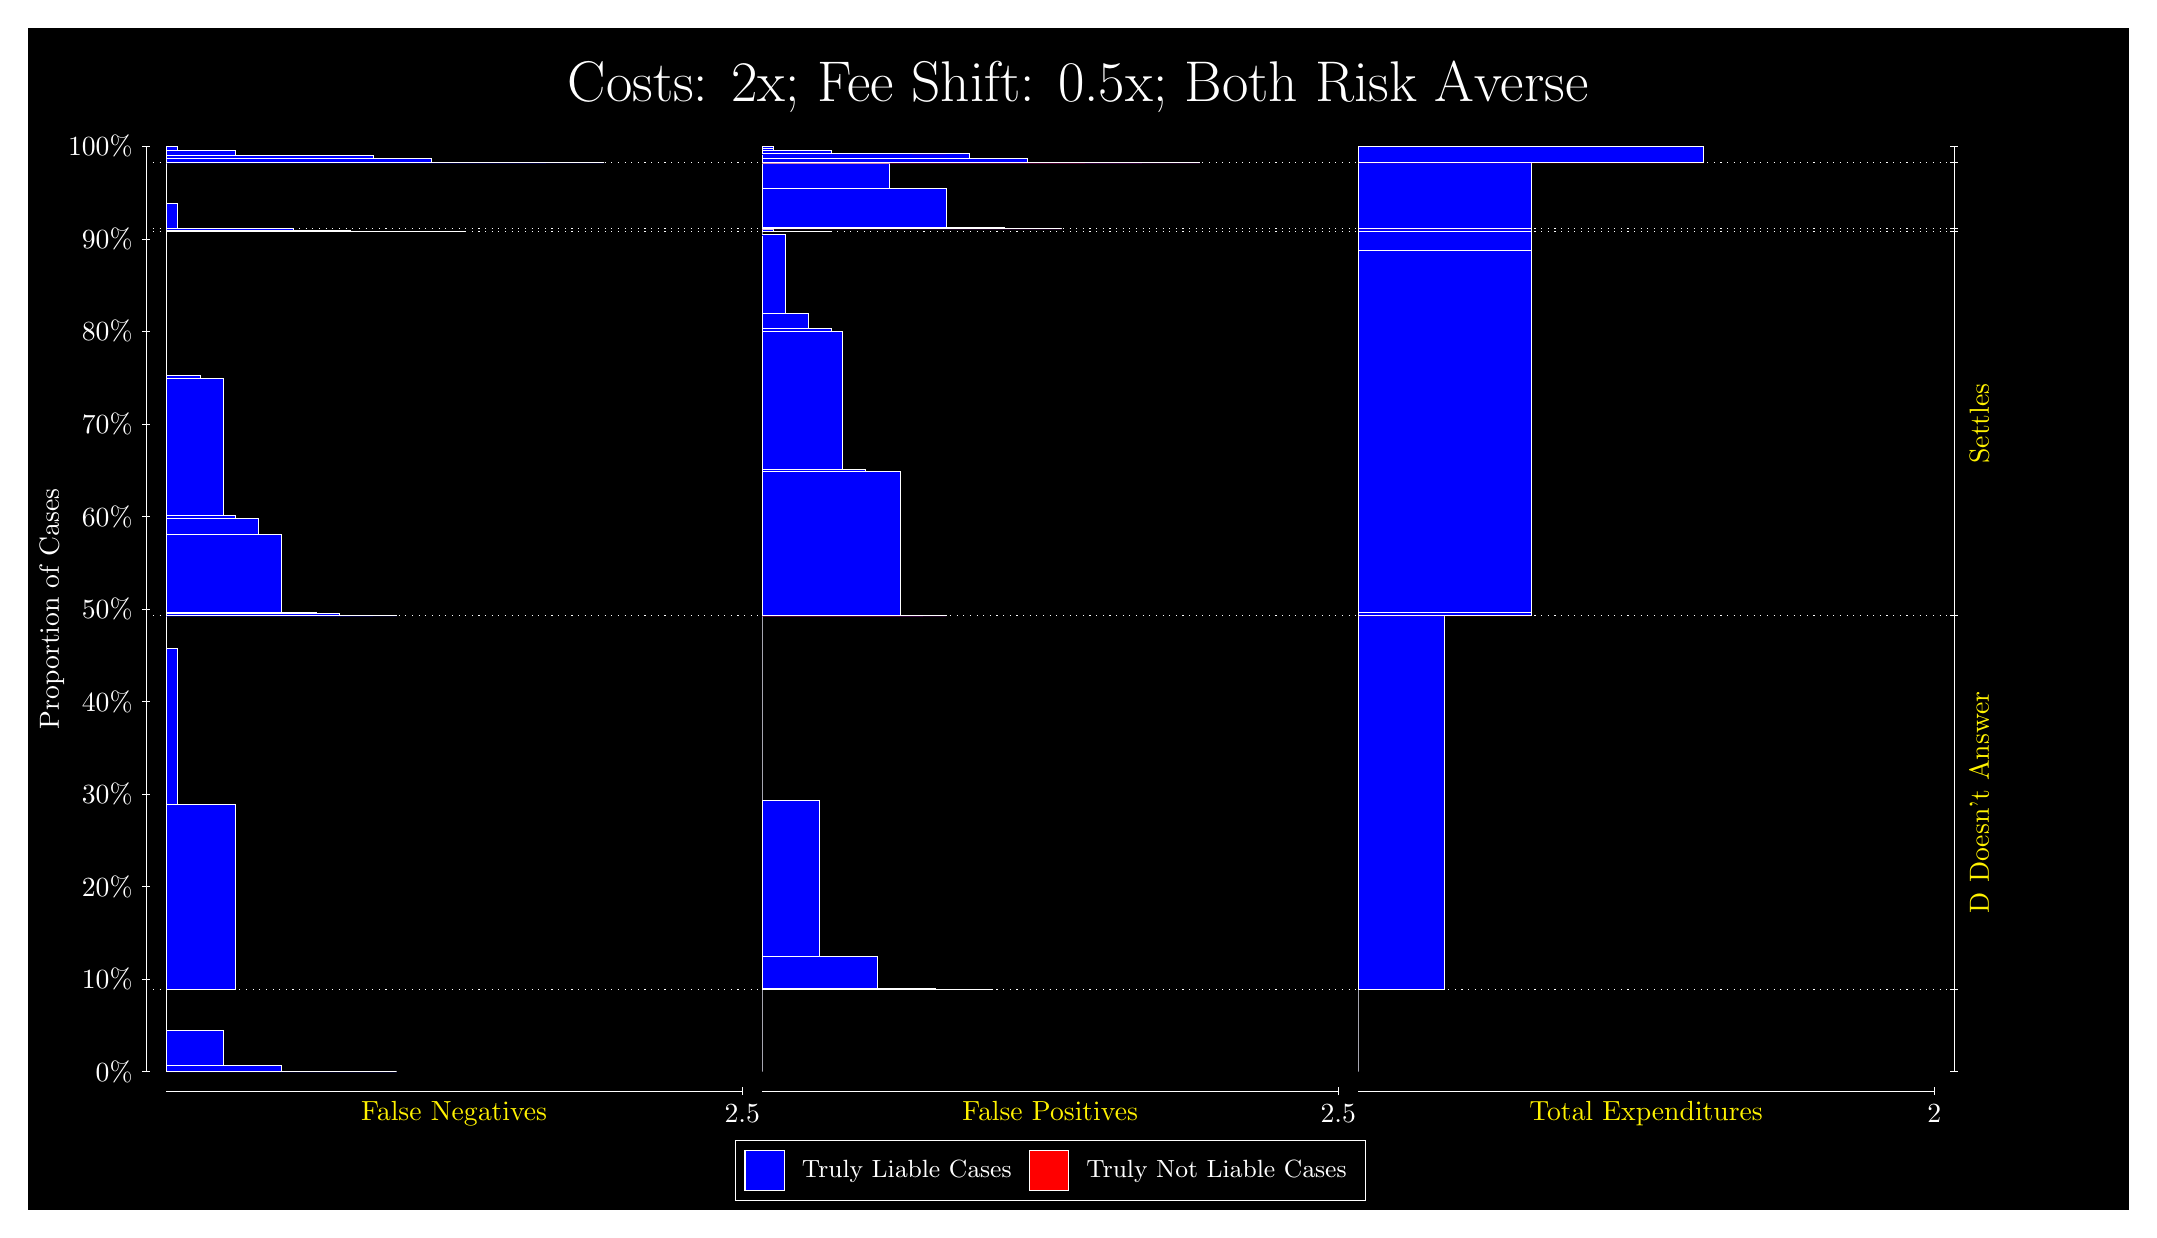
\begin{tikzpicture}
\draw[fill=black] (0,0) rectangle (26.667,15);
\draw[text=white] (0,13.5) rectangle (26.667,15) node[midway] {\huge Costs: 2x; Fee Shift: 0.5x; Both Risk Averse};
\draw[white, very thin] (1.5,1.75) -- (1.5,13.5);
\node[rotate=90, text=white, anchor=center] at (0.3, 7.625) {Proportion of Cases};
\draw[white, very thin] (1.45,1.75) -- (1.55,1.75);
\node[text=white, anchor=east] at (1.45, 1.75) {0\%};
\draw[white, very thin] (1.45,2.925) -- (1.55,2.925);
\node[text=white, anchor=east] at (1.45, 2.925) {10\%};
\draw[white, very thin] (1.45,4.1) -- (1.55,4.1);
\node[text=white, anchor=east] at (1.45, 4.1) {20\%};
\draw[white, very thin] (1.45,5.275) -- (1.55,5.275);
\node[text=white, anchor=east] at (1.45, 5.275) {30\%};
\draw[white, very thin] (1.45,6.45) -- (1.55,6.45);
\node[text=white, anchor=east] at (1.45, 6.45) {40\%};
\draw[white, very thin] (1.45,7.625) -- (1.55,7.625);
\node[text=white, anchor=east] at (1.45, 7.625) {50\%};
\draw[white, very thin] (1.45,8.8) -- (1.55,8.8);
\node[text=white, anchor=east] at (1.45, 8.8) {60\%};
\draw[white, very thin] (1.45,9.975) -- (1.55,9.975);
\node[text=white, anchor=east] at (1.45, 9.975) {70\%};
\draw[white, very thin] (1.45,11.15) -- (1.55,11.15);
\node[text=white, anchor=east] at (1.45, 11.15) {80\%};
\draw[white, very thin] (1.45,12.325) -- (1.55,12.325);
\node[text=white, anchor=east] at (1.45, 12.325) {90\%};
\draw[white, very thin] (1.45,13.5) -- (1.55,13.5);
\node[text=white, anchor=east] at (1.45, 13.5) {100\%};

\draw[white, very thin] (24.457,1.75) -- (24.457,13.5);
\draw[white, very thin] (24.407,1.75) -- (24.507,1.75);
\node[anchor=west] at (24.407, 1.75) {};
\draw[white, very thin] (24.407,2.7942) -- (24.507,2.7942);
\node[anchor=west] at (24.407, 2.7942) {};
\draw[white, very thin] (24.407,7.5411) -- (24.507,7.5411);
\node[anchor=west] at (24.407, 7.5411) {};
\draw[white, very thin] (24.407,12.42) -- (24.507,12.42);
\node[anchor=west] at (24.407, 12.42) {};
\draw[white, very thin] (24.407,12.454) -- (24.507,12.454);
\node[anchor=west] at (24.407, 12.454) {};
\draw[white, very thin] (24.407,13.293) -- (24.507,13.293);
\node[anchor=west] at (24.407, 13.293) {};
\draw[white, very thin] (24.407,13.5) -- (24.507,13.5);
\node[anchor=west] at (24.407, 13.5) {};

\draw[white, very thin, fill=blue] (1.75,1.75) rectangle (4.6775,1.75);
\draw[white, very thin, fill=blue] (1.75,1.75) rectangle (3.9457,1.7507);
\draw[white, very thin, fill=blue] (1.75,1.7507) rectangle (3.2138,1.8336);
\draw[white, very thin, fill=blue] (1.75,1.8336) rectangle (2.4819,2.2728);
\draw[white, very thin, fill=red] (1.75,2.2728) rectangle (1.75,2.2728);
\draw[white, very thin, fill=blue] (1.75,2.2728) rectangle (1.75,2.7942);
\draw[white, very thin, fill=blue] (1.75,2.7942) rectangle (2.6283,5.1405);
\draw[white, very thin, fill=blue] (1.75,5.1405) rectangle (1.8964,7.1264);
\draw[white, very thin, fill=red] (1.75,7.1264) rectangle (1.75,7.1264);
\draw[white, very thin, fill=blue] (1.75,7.1264) rectangle (1.75,7.5411);
\draw[white, very thin, fill=blue] (1.75,7.5411) rectangle (4.6775,7.5412);
\draw[white, very thin, fill=blue] (1.75,7.5412) rectangle (4.3848,7.5412);
\draw[white, very thin, fill=blue] (1.75,7.5412) rectangle (4.092,7.5412);
\draw[white, very thin, fill=blue] (1.75,7.5412) rectangle (3.9457,7.5737);
\draw[white, very thin, fill=blue] (1.75,7.5737) rectangle (3.6529,7.5833);
\draw[white, very thin, fill=blue] (1.75,7.5833) rectangle (3.3602,7.5849);
\draw[white, very thin, fill=blue] (1.75,7.5849) rectangle (3.2138,8.5785);
\draw[white, very thin, fill=blue] (1.75,8.5785) rectangle (2.921,8.7779);
\draw[white, very thin, fill=blue] (1.75,8.7779) rectangle (2.6283,8.8113);
\draw[white, very thin, fill=blue] (1.75,8.8113) rectangle (2.4819,10.559);
\draw[white, very thin, fill=blue] (1.75,10.559) rectangle (2.1891,10.589);
\draw[white, very thin, fill=blue] (1.75,10.589) rectangle (1.8964,10.594);
\draw[white, very thin, fill=red] (1.75,10.594) rectangle (1.75,10.594);
\draw[white, very thin, fill=blue] (1.75,10.594) rectangle (1.75,12.42);
\draw[white, very thin, fill=blue] (1.75,12.42) rectangle (5.5558,12.42);
\draw[white, very thin, fill=blue] (1.75,12.42) rectangle (4.8239,12.421);
\draw[white, very thin, fill=blue] (1.75,12.421) rectangle (4.092,12.432);
\draw[white, very thin, fill=blue] (1.75,12.432) rectangle (3.3602,12.454);
\draw[white, very thin, fill=blue] (1.75,12.454) rectangle (2.6283,12.454);
\draw[white, very thin, fill=red] (1.75,12.454) rectangle (1.75,12.454);
\draw[white, very thin, fill=blue] (1.75,12.454) rectangle (2.6283,12.458);
\draw[white, very thin, fill=blue] (1.75,12.458) rectangle (1.8964,12.775);
\draw[white, very thin, fill=red] (1.75,12.775) rectangle (1.75,12.775);
\draw[white, very thin, fill=blue] (1.75,12.775) rectangle (1.75,13.293);
\draw[white, very thin, fill=blue] (1.75,13.293) rectangle (7.3123,13.293);
\draw[white, very thin, fill=blue] (1.75,13.293) rectangle (6.5805,13.293);
\draw[white, very thin, fill=blue] (1.75,13.293) rectangle (5.8486,13.296);
\draw[white, very thin, fill=blue] (1.75,13.296) rectangle (5.1167,13.342);
\draw[white, very thin, fill=blue] (1.75,13.342) rectangle (4.8239,13.342);
\draw[white, very thin, fill=blue] (1.75,13.342) rectangle (4.3848,13.385);
\draw[white, very thin, fill=blue] (1.75,13.385) rectangle (4.092,13.385);
\draw[white, very thin, fill=blue] (1.75,13.385) rectangle (3.6529,13.386);
\draw[white, very thin, fill=blue] (1.75,13.386) rectangle (3.3602,13.387);
\draw[white, very thin, fill=blue] (1.75,13.387) rectangle (2.921,13.387);
\draw[white, very thin, fill=blue] (1.75,13.387) rectangle (2.6283,13.387);
\draw[white, very thin, fill=blue] (1.75,13.387) rectangle (2.6283,13.448);
\draw[white, very thin, fill=blue] (1.75,13.448) rectangle (1.8964,13.448);
\draw[white, very thin, fill=blue] (1.75,13.448) rectangle (1.8964,13.495);
\draw[white, very thin, fill=red] (1.75,13.495) rectangle (1.75,13.495);
\draw[white, very thin, fill=blue] (1.75,13.495) rectangle (1.75,13.5);
\draw[white, very thin, fill=red] (9.3189,1.75) rectangle (9.3189,1.75);
\draw[white, very thin, fill=blue] (9.3189,1.75) rectangle (9.3189,2.7942);
\draw[white, very thin, fill=red] (9.3189,2.7942) rectangle (12.246,2.7942);
\draw[white, very thin, fill=blue] (9.3189,2.7942) rectangle (12.246,2.7943);
\draw[white, very thin, fill=blue] (9.3189,2.7943) rectangle (11.515,2.8067);
\draw[white, very thin, fill=blue] (9.3189,2.8067) rectangle (10.783,3.209);
\draw[white, very thin, fill=blue] (9.3189,3.209) rectangle (10.051,5.1949);
\draw[white, very thin, fill=blue] (9.3189,5.1949) rectangle (9.3189,7.5411);
\draw[white, very thin, fill=red] (9.3189,7.5411) rectangle (11.661,7.5411);
\draw[white, very thin, fill=blue] (9.3189,7.5411) rectangle (11.661,7.5412);
\draw[white, very thin, fill=red] (9.3189,7.5412) rectangle (11.368,7.5412);
\draw[white, very thin, fill=blue] (9.3189,7.5412) rectangle (11.368,7.5412);
\draw[white, very thin, fill=red] (9.3189,7.5412) rectangle (11.075,7.5412);
\draw[white, very thin, fill=blue] (9.3189,7.5412) rectangle (11.075,9.3681);
\draw[white, very thin, fill=blue] (9.3189,9.3681) rectangle (10.929,9.3731);
\draw[white, very thin, fill=blue] (9.3189,9.3731) rectangle (10.636,9.4029);
\draw[white, very thin, fill=blue] (9.3189,9.4029) rectangle (10.344,11.15);
\draw[white, very thin, fill=blue] (9.3189,11.15) rectangle (10.197,11.184);
\draw[white, very thin, fill=blue] (9.3189,11.184) rectangle (9.9044,11.383);
\draw[white, very thin, fill=blue] (9.3189,11.383) rectangle (9.6116,12.377);
\draw[white, very thin, fill=blue] (9.3189,12.377) rectangle (9.4652,12.378);
\draw[white, very thin, fill=blue] (9.3189,12.378) rectangle (9.3189,12.42);
\draw[white, very thin, fill=red] (9.3189,12.42) rectangle (10.197,12.42);
\draw[white, very thin, fill=blue] (9.3189,12.42) rectangle (10.197,12.421);
\draw[white, very thin, fill=blue] (9.3189,12.421) rectangle (9.4652,12.442);
\draw[white, very thin, fill=blue] (9.3189,12.442) rectangle (9.3189,12.454);
\draw[white, very thin, fill=red] (9.3189,12.454) rectangle (13.125,12.454);
\draw[white, very thin, fill=blue] (9.3189,12.454) rectangle (13.125,12.454);
\draw[white, very thin, fill=blue] (9.3189,12.454) rectangle (12.393,12.468);
\draw[white, very thin, fill=blue] (9.3189,12.468) rectangle (11.661,12.973);
\draw[white, very thin, fill=blue] (9.3189,12.973) rectangle (10.929,13.289);
\draw[white, very thin, fill=blue] (9.3189,13.289) rectangle (10.197,13.293);
\draw[white, very thin, fill=red] (9.3189,13.293) rectangle (14.881,13.293);
\draw[white, very thin, fill=blue] (9.3189,13.293) rectangle (14.881,13.293);
\draw[white, very thin, fill=red] (9.3189,13.293) rectangle (14.149,13.293);
\draw[white, very thin, fill=blue] (9.3189,13.293) rectangle (14.149,13.293);
\draw[white, very thin, fill=red] (9.3189,13.293) rectangle (13.417,13.293);
\draw[white, very thin, fill=blue] (9.3189,13.293) rectangle (13.417,13.298);
\draw[white, very thin, fill=red] (9.3189,13.298) rectangle (12.686,13.298);
\draw[white, very thin, fill=blue] (9.3189,13.298) rectangle (12.686,13.346);
\draw[white, very thin, fill=blue] (9.3189,13.346) rectangle (11.954,13.406);
\draw[white, very thin, fill=red] (9.3189,13.406) rectangle (11.661,13.406);
\draw[white, very thin, fill=blue] (9.3189,13.406) rectangle (11.661,13.406);
\draw[white, very thin, fill=blue] (9.3189,13.406) rectangle (11.222,13.407);
\draw[white, very thin, fill=red] (9.3189,13.407) rectangle (10.929,13.407);
\draw[white, very thin, fill=blue] (9.3189,13.407) rectangle (10.929,13.408);
\draw[white, very thin, fill=blue] (9.3189,13.408) rectangle (10.49,13.408);
\draw[white, very thin, fill=blue] (9.3189,13.408) rectangle (10.197,13.45);
\draw[white, very thin, fill=red] (9.3189,13.45) rectangle (10.197,13.45);
\draw[white, very thin, fill=blue] (9.3189,13.45) rectangle (10.197,13.451);
\draw[white, very thin, fill=blue] (9.3189,13.451) rectangle (9.758,13.451);
\draw[white, very thin, fill=blue] (9.3189,13.451) rectangle (9.4652,13.478);
\draw[white, very thin, fill=blue] (9.3189,13.478) rectangle (9.4652,13.497);
\draw[white, very thin, fill=blue] (9.3189,13.497) rectangle (9.3189,13.5);
\draw[white, very thin, fill=red] (16.888,1.75) rectangle (16.888,1.75);
\draw[white, very thin, fill=blue] (16.888,1.75) rectangle (16.888,2.7942);
\draw[white, very thin, fill=red] (16.888,2.7942) rectangle (17.986,2.7942);
\draw[white, very thin, fill=blue] (16.888,2.7942) rectangle (17.986,7.5411);
\draw[white, very thin, fill=red] (16.888,7.5411) rectangle (19.083,7.5411);
\draw[white, very thin, fill=blue] (16.888,7.5411) rectangle (19.083,7.5812);
\draw[white, very thin, fill=red] (16.888,7.5812) rectangle (19.083,7.5812);
\draw[white, very thin, fill=blue] (16.888,7.5812) rectangle (19.083,12.182);
\draw[white, very thin, fill=red] (16.888,12.182) rectangle (19.083,12.182);
\draw[white, very thin, fill=blue] (16.888,12.182) rectangle (19.083,12.42);
\draw[white, very thin, fill=red] (16.888,12.42) rectangle (19.083,12.42);
\draw[white, very thin, fill=blue] (16.888,12.42) rectangle (19.083,12.454);
\draw[white, very thin, fill=red] (16.888,12.454) rectangle (19.083,12.454);
\draw[white, very thin, fill=blue] (16.888,12.454) rectangle (19.083,13.293);
\draw[white, very thin, fill=red] (16.888,13.293) rectangle (21.279,13.293);
\draw[white, very thin, fill=blue] (16.888,13.293) rectangle (21.279,13.5);
\draw[white, dotted] (1.5,2.7942) -- (24.457,2.7942);
\draw[white, dotted] (1.5,7.5411) -- (24.457,7.5411);
\draw[white, dotted] (1.5,12.42) -- (24.457,12.42);
\draw[white, dotted] (1.5,12.454) -- (24.457,12.454);
\draw[white, dotted] (1.5,13.293) -- (24.457,13.293);
\draw[white, very thin] (1.75,1.5) -- (9.0689,1.5);
\node[text=yellow, anchor=north] at (5.4094, 1.5) {False Negatives};
\draw[white, very thin] (9.0689,1.45) -- (9.0689,1.55);
\node[text=white, anchor=north] at (9.0689, 1.45) {2.5};

\draw[white, very thin] (9.3189,1.5) -- (16.638,1.5);
\node[text=yellow, anchor=north] at (12.978, 1.5) {False Positives};
\draw[white, very thin] (16.638,1.45) -- (16.638,1.55);
\node[text=white, anchor=north] at (16.638, 1.45) {2.5};

\draw[white, very thin] (16.888,1.5) -- (24.207,1.5);
\node[text=yellow, anchor=north] at (20.547, 1.5) {Total Expenditures};
\draw[white, very thin] (24.207,1.45) -- (24.207,1.55);
\node[text=white, anchor=north] at (24.207, 1.45) {2};


\node[text=yellow, centered, rotate=90] at (24.777, 5.1677) {D Doesn't Answer};
\node[text=yellow, centered, rotate=90] at (24.777, 9.9808) {Settles};




\draw (12.978300999999998,1.5) node[draw=none] (baseCoordinate) {};
\begin{scope}[align=center]
        \matrix[scale=0.5, draw=white, below=0.5cm of baseCoordinate, nodes={draw}, column sep=0.1cm]{
            \node[rectangle, draw, minimum width=0.5cm, minimum height=0.5cm, fill=blue] {}; &
            \node[draw=none, font=\small, text=white] (B) {Truly Liable Cases}; &
            \node[rectangle, draw, minimum width=0.5cm, minimum height=0.5cm, fill=red] {}; &
            \node[draw=none, font=\small, text=white] (B) {Truly Not Liable Cases}; \\
            };
\end{scope}

\end{tikzpicture}
\end{document}